% =====================================================================
%  Chapitre 2 -- Apprentissage supervisé : régression (2 h)
%  Introduction au Machine Learning -- CNFSDP -- L3 S5 -- 2026-2027
%  Version niveau licence (12/10/2026)
%  Compilation : pdflatex chapitre2.tex (deux fois)
%  Figures : code/figures_chapitre2.py
% =====================================================================
\documentclass[aspectratio=169,11pt]{beamer}
\usetheme{CNFSDP}
\usetikzlibrary{positioning,arrows.meta}
\usepackage{colortbl}

\chapitre{2}
\chapitrecourt{Ch.~2 \textendash{} Régression}

\title{Chapitre 2 \textendash{} Apprentissage supervisé : régression}
\subtitle{Moindres carrés, régularisation, forêts et boosting}
\author{Rois Céti DIMBAMBA}
\institute{Ingénieur statisticien économiste \textperiodcentered{} Actuaire \textperiodcentered{} \href{https://rdimbamba.shinyapps.io/roisceti_e-cv/}{\textcolor{cnfVert}{CV en ligne}}}
\date{16 octobre 2026}

\begin{document}

% ---------------------------------------------------------------------
\begin{frame}[plain,noframenumbering]
  \titlepage
\end{frame}

\begin{frame}{Plan et objectifs}
  \begin{columns}[T]
    \begin{column}{0.44\textwidth}
      \footnotesize\tableofcontents
    \end{column}
    \begin{column}{0.54\textwidth}
      \begin{objectifs}
        \footnotesize
        \begin{itemize}
          \item Écrire un modèle linéaire et l'ajuster par moindres carrés, à la main et en Python.
          \item Lire les coefficients et le $R^2$.
          \item Reconnaître le sur-apprentissage quand le modèle a trop de variables.
          \item Régulariser avec Ridge et Lasso, et choisir la pénalité.
          \item Utiliser forêts aléatoires et gradient boosting en régression.
        \end{itemize}
      \end{objectifs}
      \vskip-1mm{\scriptsize\color{cnfGris}Prérequis : chapitre~0 (droite des moindres carrés, gradient, matrices) et chapitre~1 (risque, validation croisée).}
    \end{column}
  \end{columns}
\end{frame}

% =====================================================================
\section{Le problème de régression}

\begin{frame}{Prédire une quantité}
  \begin{definition}[Problème de régression]
    Un problème supervisé est un problème de \emph{régression} quand la cible $y$ est un nombre réel.
    On mesure l'erreur par la perte quadratique : le risque d'un prédicteur $f$ est $R(f)=\E\big[(Y-f(X))^2\big]$.
  \end{definition}
  {\small Exemples : revenu d'un ménage, nombre d'enfants d'une femme, rendement d'une parcelle, durée d'un chômage.}
  \vskip2mm
  \begin{columns}[T]
    \begin{column}{0.46\textwidth}
      \small
      \textbf{Fil rouge} (chiffres fictifs) : $5$ femmes.
      \vskip1mm
      \renewcommand{\arraystretch}{1.15}
      \begin{tabular}{lccccc}
        \toprule
        années d'études $x$ & $0$ & $3$ & $6$ & $9$ & $12$ \\
        nombre d'enfants $y$ & $6$ & $5$ & $5$ & $3$ & $1$ \\
        \bottomrule
      \end{tabular}
    \end{column}
    \begin{column}{0.5\textwidth}
      \begin{remarque}[Rappel du chapitre 1]
        Le meilleur prédicteur possible est la moyenne conditionnelle $f^*(x)=\E[Y\mid X=x]$.
        Elle est inconnue : on cherche à l'approcher à partir des données.
      \end{remarque}
    \end{column}
  \end{columns}
\end{frame}

\begin{frame}{Le modèle linéaire}
  \begin{definition}[Prédicteur linéaire]
    Avec $d$ variables explicatives $x=(x_1,\dots,x_d)$, un \emph{prédicteur linéaire} est de la forme
    \[
      f_\theta(x)=\theta_0+\theta_1x_1+\dots+\theta_dx_d ,
    \]
    où $\theta=(\theta_0,\theta_1,\dots,\theta_d)$ sont les \emph{coefficients} : $\theta_0$ est la constante, $\theta_j$ l'effet de la variable $x_j$.
  \end{definition}
  \begin{itemize}\small
    \item \textbf{Simple} : $d+1$ nombres à estimer, que l'on peut interpréter.
    \item \textbf{Souvent une bonne approximation} de $\E[Y\mid X=x]$, au moins localement.
    \item \textbf{Plus souple qu'il n'y paraît} : on peut y mettre $x^2$, $\log(\text{revenu})$, des indicatrices de catégories\dots{} « Linéaire » veut dire linéaire \emph{en $\theta$}.
  \end{itemize}
\end{frame}

% =====================================================================
\section{Les moindres carrés}

\begin{frame}{Moindres carrés avec une variable}
  \small
  \begin{definition}[Estimateur des moindres carrés ordinaires (MCO)]
    Les coefficients $(\hat a,\hat b)$ des MCO sont ceux qui minimisent le risque empirique quadratique
    \[
      \Rn(a,b)=\frac1n\sum_{i=1}^n\big(y_i-a-bx_i\big)^2 .
    \]
  \end{definition}
  \begin{proposition}[droite des moindres carrés, chapitre 0]
    Avec $s_{xy}=\frac1n\sum_i(x_i-\bar x)(y_i-\bar y)$ et $s_x^2=\frac1n\sum_i(x_i-\bar x)^2>0$,
    \[
      \hat b=s_{xy}/s_x^2,\qquad \hat a=\bar y-\hat b\,\bar x .
    \]
  \end{proposition}
  \begin{preuve}[(rappel)]
    $\partial\Rn/\partial a=0$ donne $a=\bar y-b\bar x$ ; il reste $s_y^2-2b\,s_{xy}+b^2s_x^2$, minimal en $b=s_{xy}/s_x^2$.
  \end{preuve}
\end{frame}

\begin{frame}{Le calcul sur le fil rouge}
  \begin{columns}[T]
    \begin{column}{0.55\textwidth}
      \small
      $\bar x=6$, $\bar y=4$.
      \vskip1mm
      \renewcommand{\arraystretch}{1.12}
      \begin{tabular}{rrrrrr}
        \toprule
        $x_i$ & $y_i$ & $x_i-\bar x$ & $y_i-\bar y$ & produit & carré \\
        \midrule
        $0$ & $6$ & $-6$ & $2$ & $-12$ & $36$ \\
        $3$ & $5$ & $-3$ & $1$ & $-3$ & $9$ \\
        $6$ & $5$ & $0$ & $1$ & $0$ & $0$ \\
        $9$ & $3$ & $3$ & $-1$ & $-3$ & $9$ \\
        $12$ & $1$ & $6$ & $-3$ & $-18$ & $36$ \\
        \midrule
        \multicolumn{4}{r}{moyenne} & $s_{xy}=-7{,}2$ & $s_x^2=18$ \\
        \bottomrule
      \end{tabular}
      \vskip2mm
      $\hat b=\frac{-7{,}2}{18}=-0{,}4$ \quad et \quad $\hat a=4-(-0{,}4)\times6=6{,}4$.
    \end{column}
    \begin{column}{0.43\textwidth}
      \centering
      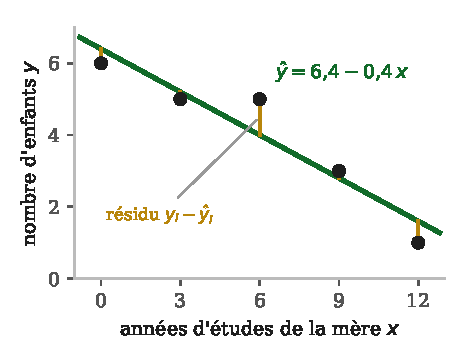
\includegraphics[width=\textwidth]{droite.pdf}
    \end{column}
  \end{columns}
  \vskip1mm
  \begin{remarque}[Lecture]
    Une année d'études de plus est associée, en moyenne, à $0{,}4$ enfant de moins. C'est une \emph{association} observée, pas un effet causal démontré.
  \end{remarque}
\end{frame}

\begin{frame}{Résidus et coefficient de détermination}
  \begin{definition}[Résidus, $R^2$]
    Les \emph{résidus} sont $e_i=y_i-\hat y_i$, où $\hat y_i=\hat a+\hat bx_i$. Le \emph{coefficient de détermination} est
    \[
      R^2=1-\frac{\sum_ie_i^2}{\sum_i(y_i-\bar y)^2}\in[0,1].
    \]
  \end{definition}
  \small
  \begin{itemize}
    \item Les résidus des MCO sont de somme nulle : c'est l'équation $\partial\Rn/\partial a=0$.
    \item Fil rouge : $\hat y=(6{,}4;\,5{,}2;\,4;\,2{,}8;\,1{,}6)$, résidus $(-0{,}4;\,-0{,}2;\,1;\,0{,}2;\,-0{,}6)$, de somme nulle.
    \item $\sum_ie_i^2=1{,}6$ et $\sum_i(y_i-\bar y)^2=16$, d'où $R^2=1-\frac{1{,}6}{16}=0{,}9$.
  \end{itemize}
  \begin{remarque}[Lecture et piège]
    La droite « explique » $90\,\%$ de la dispersion du nombre d'enfants. Mais ce $R^2$ est calculé sur les données d'apprentissage : il augmente toujours quand on ajoute des variables. On juge un modèle sur un échantillon test (chapitre~1).
  \end{remarque}
\end{frame}

% =====================================================================
\section{Plusieurs variables}

\begin{frame}{L'écriture matricielle}
  On range les données dans une matrice $X$ à $n$ lignes et $d+1$ colonnes, la première colonne étant remplie de $1$ (pour la constante), et les cibles dans un vecteur $y\in\R^n$.
  Les prédictions s'écrivent $\hat y=X\theta$ et le risque empirique
  \[
    \Rn(\theta)=\frac1n\norm{y-X\theta}^2=\frac1n\sum_{i=1}^n\big(y_i-\theta_0-\theta_1x_{i1}-\dots-\theta_dx_{id}\big)^2 .
  \]
  \begin{theoreme}[Moindres carrés : équations normales]
    Si la matrice $X\T X$ est inversible, le risque empirique atteint son minimum en un unique point,
    \[
      \hat\theta=(X\T X)^{-1}X\T y .
    \]
  \end{theoreme}
  \begin{preuve}[(idée)]
    Au minimum, le gradient est nul : $\nabla\Rn(\theta)=-\frac2nX\T(y-X\theta)=0$, soit $X\T X\,\theta=X\T y$ (calcul du gradient admis).
  \end{preuve}
\end{frame}

\begin{frame}{Vérification sur le fil rouge}
  \small
  \[
    X=\begin{pmatrix}1&0\\1&3\\1&6\\1&9\\1&12\end{pmatrix},\quad
    X\T X=\begin{pmatrix}5&30\\30&270\end{pmatrix},\quad
    X\T y=\begin{pmatrix}\sum y_i\\\sum x_iy_i\end{pmatrix}=\begin{pmatrix}20\\84\end{pmatrix}.
  \]
  Le déterminant vaut $5\times270-30\times30=450$, donc (chapitre~0)
  \[
    (X\T X)^{-1}=\frac1{450}\begin{pmatrix}270&-30\\-30&5\end{pmatrix},\qquad
    \hat\theta=\frac1{450}\begin{pmatrix}270\times20-30\times84\\-30\times20+5\times84\end{pmatrix}=\begin{pmatrix}6{,}4\\-0{,}4\end{pmatrix}.
  \]
  \begin{aretenir}
    Avec une seule variable, la formule matricielle redonne la droite des moindres carrés. Avec $d$ variables, c'est le même calcul : l'ordinateur résout le système $X\T X\theta=X\T y$.
  \end{aretenir}
\end{frame}

\begin{frame}{Lire les coefficients}
  \begin{definition}[Interprétation d'un coefficient]
    $\hat\theta_j$ est la variation moyenne de la prédiction quand $x_j$ augmente d'une unité, \emph{les autres variables restant fixées}.
  \end{definition}
  \vskip2mm
  \begin{columns}[T]
    \begin{column}{0.5\textwidth}
      \small
      \textbf{Variable qualitative.} On la code par des \emph{indicatrices}, en laissant une catégorie de référence :
      \[
        x_{\text{rural}}=\begin{cases}1&\text{si rural}\\0&\text{si urbain.}\end{cases}
      \]
      Dans $\hat y=\hat\theta_0+\hat\theta_1\,\text{études}+\hat\theta_2\,x_{\text{rural}}$, le coefficient $\hat\theta_2$ est l'écart moyen entre rurales et urbaines \emph{à niveau d'études égal}.
    \end{column}
    \begin{column}{0.46\textwidth}
      \begin{remarque}[Précautions]
        \begin{itemize}\setlength\itemsep{1pt}
          \item Un coefficient dépend de l'unité de $x_j$ (années, mois, FCFA).
          \item Il dépend aussi des autres variables présentes dans le modèle.
          \item Association n'est pas causalité.
        \end{itemize}
      \end{remarque}
    \end{column}
  \end{columns}
\end{frame}

% =====================================================================
\section{Quand les moindres carrés déraillent}

\begin{frame}{Trop de variables : le sur-apprentissage revient}
  \centering
  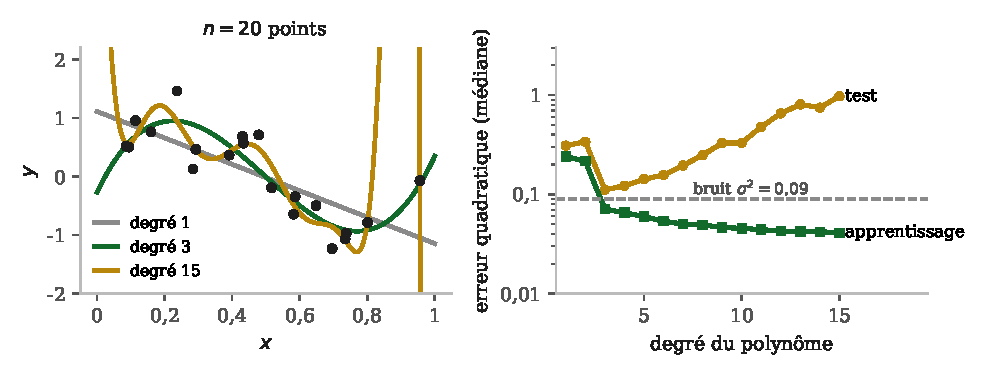
\includegraphics[width=0.74\textwidth]{polynome.pdf}
  \vskip1mm
  \begin{minipage}{0.94\textwidth}
    \small
    $Y=\sin(2\pi X)+\varepsilon$, $\sigma=0{,}3$ ; polynômes de degré $1$ à $15$ (variables $x,x^2,\dots,x^d$) ajustés par MCO.
    Le degré $1$ est trop rigide, le degré $3$ est le meilleur sur le test ; le degré $15$ colle aux points et oscille entre eux : l'erreur test explose.
    \vskip1mm
    {\color{cnfGris}Autres symptômes : si $d+1>n$, $X\T X$ n'est pas inversible (une infinité de solutions annulent l'erreur d'apprentissage) ; si deux variables sont très corrélées, leurs coefficients deviennent instables.}
  \end{minipage}
\end{frame}

% =====================================================================
\section{Régulariser : Ridge et Lasso}

\begin{frame}{La régression Ridge}
  \begin{definition}[Ridge]
    Pour une pénalité $\lambda\ge0$, les coefficients Ridge minimisent
    \[
      \frac1n\sum_{i=1}^n\big(y_i-\theta_0-\theta_1x_{i1}-\dots-\theta_dx_{id}\big)^2+\lambda\sum_{j=1}^d\theta_j^2 .
    \]
  \end{definition}
  \begin{itemize}\small
    \item Le premier terme veut coller aux données, le second veut des coefficients petits. On ne pénalise pas la constante $\theta_0$.
    \item $\lambda=0$ : on retrouve les MCO. Quand $\lambda$ grandit, les $\hat\theta_j$ se rapprochent de $0$.
    \item La solution existe et est unique pour tout $\lambda>0$, même si $d+1>n$ (admis).
  \end{itemize}
  \begin{aretenir}
    Régulariser, c'est accepter un peu de biais pour réduire beaucoup la variance (chapitre~1).
  \end{aretenir}
\end{frame}

\begin{frame}{Ridge avec une variable : un calcul complet}
  \begin{proposition}
    Avec une seule variable, la pente Ridge vaut
    \[
      \hat b_\lambda=\frac{s_{xy}}{s_x^2+\lambda},\qquad\text{et}\qquad\hat a_\lambda=\bar y-\hat b_\lambda\,\bar x .
    \]
  \end{proposition}
  \begin{preuve}
    La pénalité ne dépend pas de $a$ : comme pour les MCO, $a=\bar y-b\bar x$. Il reste à minimiser
    $s_y^2-2b\,s_{xy}+b^2s_x^2+\lambda b^2$, dont la dérivée $-2s_{xy}+2b\,(s_x^2+\lambda)$ s'annule en $b=s_{xy}/(s_x^2+\lambda)$.
  \end{preuve}
  \begin{exemple}[Fil rouge]
    $s_{xy}=-7{,}2$, $s_x^2=18$. Pour $\lambda=4$ : $\hat b_4=\frac{-7{,}2}{22}\approx-0{,}327$ au lieu de $-0{,}4$.
    Le dénominateur grossit : la pente est \emph{rétrécie} vers $0$, sans jamais l'atteindre.
  \end{exemple}
\end{frame}

\begin{frame}{La régression Lasso}
  \small
  \begin{definition}[Lasso]
    Les coefficients Lasso minimisent le même critère que Ridge, avec $\lambda\sum_{j=1}^d|\theta_j|$ à la place de $\lambda\sum_{j=1}^d\theta_j^2$ : on pénalise les valeurs absolues au lieu des carrés.
  \end{definition}
  \begin{proposition}[admise]
    Avec une seule variable,
    $\hat b_\lambda=\operatorname{signe}(s_{xy})\times\dfrac{\max\big(|s_{xy}|-\lambda/2,\;0\big)}{s_x^2}$ : la pente est \emph{exactement nulle} dès que $\lambda\ge2|s_{xy}|$.
  \end{proposition}
  \begin{center}
    \small\renewcommand{\arraystretch}{1.05}
    \begin{tabular}{lccccc}
      \toprule
      $\lambda$ & $0$ & $4$ & $10$ & $14{,}4$ & $20$ \\
      \midrule
      pente Ridge & $-0{,}400$ & $-0{,}327$ & $-0{,}257$ & $-0{,}222$ & $-0{,}189$ \\
      pente Lasso & $-0{,}400$ & $-0{,}289$ & $-0{,}122$ & $\mathbf{0}$ & $\mathbf{0}$ \\
      \bottomrule
    \end{tabular}
  \end{center}
  {\small\color{cnfGris}Ridge rétrécit tous les coefficients ; Lasso en annule certains : il \emph{sélectionne} les variables.}
\end{frame}

\begin{frame}{Les chemins de régularisation}
  \centering
  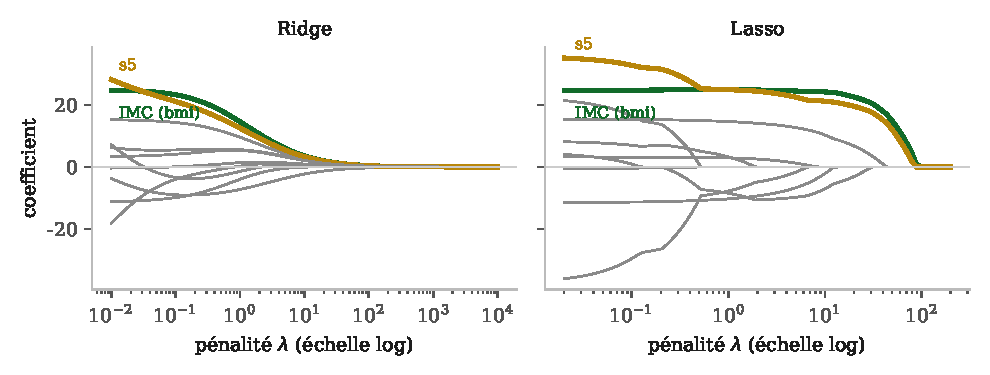
\includegraphics[width=0.84\textwidth]{chemins.pdf}
  \vskip1mm
  \begin{minipage}{0.92\textwidth}
    \small
    Données \texttt{diabetes} de scikit-learn : $442$ patients, $10$ variables standardisées (âge, sexe, IMC, tension, $6$ mesures sanguines \texttt{s1} à \texttt{s6}) ; $y$ = progression de la maladie un an plus tard.
    Chaque courbe suit un coefficient quand $\lambda$ augmente. Avec le Lasso, les coefficients s'annulent un à un : vers $\lambda=40$, il ne reste que $3$ variables : l'IMC, la tension (\texttt{bp}) et \texttt{s5}.
  \end{minipage}
\end{frame}

\begin{frame}{Bien utiliser Ridge et Lasso}
  \begin{enumerate}
    \item \textbf{Standardiser les variables} (moyenne $0$, écart type $1$) : la pénalité compare des coefficients, qui dépendent des unités. Un revenu en FCFA ou en millions de FCFA ne serait pas pénalisé de la même façon.
    \item \textbf{Choisir $\lambda$ par validation croisée} (chapitre~1) : pour chaque $\lambda$ d'une grille, on calcule l'erreur de validation croisée ; on garde le $\lambda$ qui la minimise, puis on réapprend sur tout l'échantillon d'apprentissage.
    \item \textbf{Choisir la pénalité} : Ridge si beaucoup de variables utiles et corrélées ; Lasso si l'on pense que peu de variables comptent, ou pour un modèle plus lisible.
  \end{enumerate}
  \begin{remarque}[Conventions de scikit-learn]
    Le paramètre s'appelle \texttt{alpha}, avec d'autres échelles : \texttt{Ridge(alpha=}$n\lambda$\texttt{)} et \texttt{Lasso(alpha=}$\lambda/2$\texttt{)}. \texttt{RidgeCV} et \texttt{LassoCV} font la validation croisée.
  \end{remarque}
\end{frame}

% =====================================================================
\section{Arbres, forêts et boosting}

\begin{frame}{L'arbre de régression}
  \begin{definition}[Arbre de régression]
    Un arbre découpe l'espace des $x$ en zones par des questions du type « $x_j\le s$ ? ». Dans chaque zone (\emph{feuille}), il prédit la \emph{moyenne} des $y_i$ de la zone : la meilleure constante (chapitre~1).
  \end{definition}
  \begin{columns}[T]
    \begin{column}{0.5\textwidth}
      \small
      \textbf{Choisir la coupure.} On essaie chaque seuil et l'on garde celui qui minimise la somme des carrés des écarts à la moyenne, dans les deux zones.
      \vskip1mm
      Fil rouge, une seule coupure : on retient $x\le7{,}5$. L'arbre prédit $\frac{6+5+5}3\approx5{,}33$ enfants à gauche et $\frac{3+1}2=2$ à droite.
    \end{column}
    \begin{column}{0.46\textwidth}
      \small\centering
      \renewcommand{\arraystretch}{1.15}
      \begin{tabular}{lcc}
        \toprule
        seuil & zones & somme des carrés \\
        \midrule
        $1{,}5$ & $\{6\}\,|\,\{5,5,3,1\}$ & $11$ \\
        $4{,}5$ & $\{6,5\}\,|\,\{5,3,1\}$ & $8{,}5$ \\
        $7{,}5$ & $\{6,5,5\}\,|\,\{3,1\}$ & $\mathbf{2{,}67}$ \\
        $10{,}5$ & $\{6,5,5,3\}\,|\,\{1\}$ & $4{,}75$ \\
        \bottomrule
      \end{tabular}
    \end{column}
  \end{columns}
  \vskip2mm
  {\small\color{cnfGris}On recommence dans chaque zone. Un arbre profond sur-apprend (chapitre~1) : il est très \emph{instable}.}
\end{frame}

\begin{frame}{Forêt aléatoire : la moyenne de nombreux arbres}
  \begin{definition}[Bagging, forêt aléatoire]
    \begin{enumerate}\setlength\itemsep{1pt}
      \item On tire $B$ échantillons \emph{bootstrap} : $n$ individus tirés \emph{avec remise} dans l'échantillon.
      \item Sur chacun, on apprend un arbre profond $\hat f_b$.
      \item On prédit par la moyenne $\hat f(x)=\frac1B\sum_{b=1}^B\hat f_b(x)$.
    \end{enumerate}
    Une \emph{forêt aléatoire} ajoute du hasard : à chaque coupure, l'arbre ne regarde qu'une partie des variables, tirée au sort.
  \end{definition}
  \begin{itemize}\small
    \item Chaque arbre est instable, mais leurs erreurs se compensent : la moyenne varie beaucoup moins (calcul au chapitre~3).
    \item Réglages : nombre d'arbres $B$ (plusieurs centaines), taille minimale des feuilles, nombre de variables tirées.
  \end{itemize}
\end{frame}

\begin{frame}{Gradient boosting : corriger pas à pas}
  \begin{definition}[Gradient boosting en régression]
    On part de $F_0(x)=\bar y$. Pour $m=1,\dots,M$ :
    \begin{enumerate}\setlength\itemsep{1pt}
      \item on calcule les résidus $r_i=y_i-F_{m-1}(x_i)$ : ce qui reste à expliquer ;
      \item on ajuste un \emph{petit} arbre $h_m$ sur les couples $(x_i,r_i)$ ;
      \item on corrige un peu : $F_m(x)=F_{m-1}(x)+\nu\,h_m(x)$, avec un taux d'apprentissage $0<\nu\le1$.
    \end{enumerate}
  \end{definition}
  \small
  \textbf{Fil rouge}, arbres à une coupure, $\nu=0{,}5$ : $F_0=4$ ; résidus $(2;1;1;-1;-3)$.
  Le meilleur arbre coupe en $x\le7{,}5$ et prédit $\frac43$ à gauche, $-2$ à droite.
  \[
    F_1=(4{,}67;\;4{,}67;\;4{,}67;\;3;\;3),\qquad F_2=(4{,}92;\;4{,}92;\;4{,}92;\;3{,}25;\;2)\quad\text{pour }y=(6;5;5;3;1).
  \]
\end{frame}

\begin{frame}{Bagging et boosting en image}
  \centering
  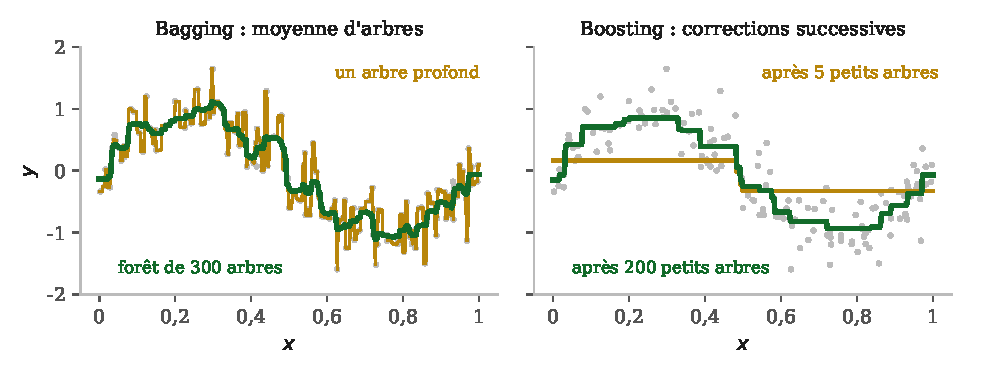
\includegraphics[width=0.74\textwidth]{ensembles.pdf}
  \vskip1mm
  \small\renewcommand{\arraystretch}{1.15}
  \begin{tabular}{p{0.2\textwidth}p{0.34\textwidth}p{0.36\textwidth}}
    \toprule
    & \textbf{Forêt (bagging)} & \textbf{Gradient boosting} \\
    \midrule
    Arbres & profonds, appris en parallèle & petits, appris l'un après l'autre \\
    Ce qui baisse & la variance & le biais \\
    Réglages clés & $B$, taille des feuilles & $\nu$, nombre d'arbres $M$, profondeur \\
    \bottomrule
  \end{tabular}
\end{frame}

\begin{frame}{Quel modèle choisir ?}
  \small
  \renewcommand{\arraystretch}{1.3}
  \begin{tabular}{p{0.2\textwidth}p{0.36\textwidth}p{0.36\textwidth}}
    \toprule
    \textbf{Modèle} & \textbf{Points forts} & \textbf{Limites} \\
    \midrule
    MCO & simple, rapide, coefficients lisibles & sur-apprend avec beaucoup de variables \\
    Ridge, Lasso & beaucoup de variables, variables corrélées ; Lasso sélectionne & relation supposée linéaire ; standardiser \\
    Forêt, boosting & relations non linéaires, interactions, peu de préparation & moins lisibles ; demandent plus de données \\
    \bottomrule
  \end{tabular}
  \vskip3mm
  \begin{aretenir}
    Aucun modèle ne gagne toujours. Sur une relation en sinus, la forêt et le boosting font nettement mieux que la droite (erreur $0{,}32$ contre $0{,}54$) ; sur les données \texttt{diabetes}, la régression linéaire bat la forêt. On compare toujours sur un échantillon test ou par validation croisée.
  \end{aretenir}
\end{frame}

% =====================================================================
\section{En Python}

\begin{frame}[fragile]{Moindres carrés : à la main puis avec scikit-learn}
\begin{python}
import numpy as np
from sklearn.linear_model import LinearRegression

# Fil rouge : années d'études de la mère (x), nombre d'enfants (y)
x = np.array([0, 3, 6, 9, 12]); y = np.array([6, 5, 5, 3, 1])
X = np.column_stack([np.ones(5), x])            # colonne de 1 pour la constante
theta = np.linalg.solve(X.T @ X, X.T @ y)       # équations normales
print(theta)                                    # [ 6.4 -0.4]

f = LinearRegression().fit(x.reshape(-1, 1), y) # même calcul avec scikit-learn
print(f.intercept_, f.coef_)                    # 6.4 [-0.4]
print(round(f.score(x.reshape(-1, 1), y), 3))   # R² = 0.9
\end{python}
\vskip-1mm
{\small\color{cnfGris}\texttt{np.linalg.solve} résout le système $X\T X\theta=X\T y$ sans calculer l'inverse, ce qui est plus précis.}
\end{frame}

\begin{frame}[fragile]{Ridge et Lasso avec validation croisée}
\begin{python}[basicstyle=\ttfamily\scriptsize]
from sklearn.datasets import load_diabetes
from sklearn.model_selection import train_test_split
from sklearn.pipeline import make_pipeline
from sklearn.preprocessing import StandardScaler
from sklearn.linear_model import LinearRegression, RidgeCV, LassoCV
from sklearn.metrics import root_mean_squared_error

X, y = load_diabetes(return_X_y=True, as_frame=True)   # 442 patients, 10 variables
Xa, Xt, ya, yt = train_test_split(X, y, test_size=0.3, random_state=0)
modeles = {"MCO": LinearRegression(),
           "Ridge": RidgeCV(alphas=np.logspace(-3, 3, 50)),
           "Lasso": LassoCV(cv=5, random_state=0)}
for nom, m in modeles.items():
    f = make_pipeline(StandardScaler(), m).fit(Xa, ya)  # standardiser puis ajuster
    print(nom, round(root_mean_squared_error(yt, f.predict(Xt)), 1))
coef = f[-1].coef_                                       # coefficients du Lasso
print(list(X.columns[coef == 0]))                        # variables écartées
# MCO 55.7 | Ridge 55.4 | Lasso 55.8 | écartées : ['s2', 's4', 's6']
\end{python}
\vskip-1mm
{\small\color{cnfGris}Les trois se valent (environ $55$ points d'erreur) ; le Lasso n'utilise que $7$ variables sur $10$.}
\end{frame}

\begin{frame}[fragile]{Forêt et boosting contre la régression linéaire}
\begin{python}[basicstyle=\ttfamily\scriptsize]
from sklearn.ensemble import RandomForestRegressor, GradientBoostingRegressor
rng = np.random.default_rng(0)

def simuler(n):                                     # relation non linéaire
    x = rng.uniform(0, 1, (n, 1))
    return x, np.sin(2 * np.pi * x[:, 0]) + 0.3 * rng.standard_normal(n)

X, y = simuler(300); Xt, yt = simuler(5_000)
modeles = {
    "linéaire": LinearRegression(),
    "forêt": RandomForestRegressor(n_estimators=200, min_samples_leaf=5,
                                   random_state=0),
    "boosting": GradientBoostingRegressor(n_estimators=200, learning_rate=0.05,
                                          max_depth=2, random_state=0)}
for nom, f in modeles.items():
    print(nom, round(root_mean_squared_error(yt, f.fit(X, y).predict(Xt)), 3))
# linéaire 0.541 | forêt 0.316 | boosting 0.317
\end{python}
\vskip-1mm
{\small\color{cnfGris}Le bruit a pour écart type $\sigma=0{,}3$ : la forêt et le boosting en sont tout près, la droite non.}
\end{frame}

% =====================================================================
\section{TP en salle}

\begin{frame}{TP2 \textendash{} Moindres carrés, régularisation, ensembles}
  \footnotesize
  \begin{tp}{TP2 \textendash{} à faire en salle}{30 min \textperiodcentered{} \texttt{notebooks/TP2.ipynb} (Colab)}
    \begin{enumerate}\setlength\itemsep{1pt}
      \item \textbf{Moindres carrés.} Simuler $n=100$ points de $Y=2+3X+\varepsilon$ ; calculer $\hat a$, $\hat b$ par les formules, puis par les équations normales ; comparer avec \texttt{LinearRegression} et calculer le $R^2$.
      \item \textbf{Chemin du Lasso} (données \texttt{diabetes}) : quelles variables restent quand $\lambda$ grandit ?
      \item \textbf{Choix de $\lambda$} par validation croisée ; comparer les erreurs test des MCO, de Ridge et du Lasso.
      \item \textbf{Boosting à la main} : programmer deux étapes sur le fil rouge et retrouver $F_1$ et $F_2$ du cours.
      \item \textbf{Ensembles} : comparer régression linéaire, forêt et gradient boosting sur la relation en sinus, puis sur \texttt{diabetes}.
    \end{enumerate}
  \end{tp}
\end{frame}

\begin{frame}{Résumé}
  \begin{itemize}
    \item Régression : prédire un nombre ; on approche $\E[Y\mid X=x]$ en minimisant l'erreur quadratique.
    \item Moindres carrés : $\hat b=s_{xy}/s_x^2$ avec une variable, $\hat\theta=(X\T X)^{-1}X\T y$ en général ; le $R^2$ mesure l'ajustement, pas la qualité de prédiction.
    \item Avec trop de variables, les MCO sur-apprennent et deviennent instables.
    \item Ridge rétrécit les coefficients, Lasso en annule certains ; on standardise et l'on choisit $\lambda$ par validation croisée.
    \item Arbres : moyenne par zone. Forêt : moyenne d'arbres (moins de variance). Boosting : petits arbres qui corrigent les résidus (moins de biais).
    \item Aucun modèle n'est toujours le meilleur : on compare sur des données test.
  \end{itemize}
\end{frame}

\end{document}
